In this section, we provide the big picture view of the complete Pandora $\nu_e$ analysis, starting from our selection philosophy and ending with our strategy regarding systematic uncertainties. A broad summary of the current status of the analysis is presented in section~\ref{sec:introduction:conclusions}. Each topic is discussed in more detail in subsequent chapters of this document.  This chapter should provide a brief but complete overview of the analysis, including its main results.

\subsection{$\nu_e$ Selection Philosophy} %\textcolor{green}{David ... (P.R. Elena,Sophie) }
\par Several proposals have been made to explain the nature of the MiniBooNE LEE anomaly. It is fair to say that a large amount of uncertainty remains in the community regarding what may have generated such an excess of electromagnetic events. This analysis works within the $\nu_e$ excess hypothesis.  To best explore the potential new physics in the $\nu_e$ channel at low energy, this analysis aims to perform an inclusive multi-channel measurement of $\nu_e$ interactions without relying on the kinematic variables which depend on neutrino-interaction models. A multi-channel approach can reduce systematic uncertainties associated with the chosen interaction model in addition to building stronger confidence against mis-modeling of neutrino interaction and detector simulations. Finally, such a search allows the analysis to be sensitive to a broader range of possible new-physics explanations for a low-energy-excess.

\par This analysis relies on two exclusive and orthogonal selections to isolate $\nu_e$ interactions and be sensitive to new physics at low energy. The two channels, both requiring no final state pions, differ by the presence or lack of final-state protons and are denoted in this note by their final-state topology as \npsel and \zpsel respectively. These two channels combined match the MiniBooNE signal channel (1$e$X$p$0$\pi$). An inclusive $\nu_e$ selection is currently developed independently of the other two selections; while it is not an input to the analysis sensitivity, it provides an important sideband capable of measuring $\nu_e$ interactions above $\sim$700 MeV with high statistics and thus help study the modeling of $\nu_e$ kinematics modeling in this energy regime. A schematic summarizing the strengths and features of each selection is shown in Table~\ref{tab:selectionsNue}. 
%\textcolor{red}{Should we add that our main selection is the 1$e$N$p$0$\pi$? }

\begin{table}[ht]
\caption{\label{tab:selectionsNue} Schematic of the three $\nu_e$ selections, outlining the definition and goals of each. In this work, the threshold for a visible proton at truth-level is 40 MeV of kinetic energy (KE). N refers to one or more, and X to any number of final state particles of a given category.}
\centering
\begin{tabular}{ m{0.1\textwidth} | m{0.2\textwidth}  m{0.45\textwidth}  }
Channel & Description & Goal \\
\hline
 \begin{center}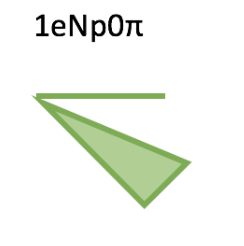
\includegraphics[width=0.1\textwidth]{introduction/1eNp}\end{center}& At least one visible proton and no visible pions & Most sensitive channel to MiniBooNE unfolded signal. The presence of a proton facilitates vertex finding.\\
\hline
 \begin{center}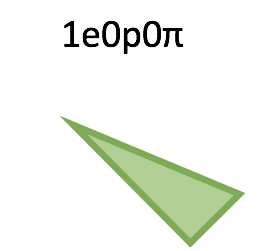
\includegraphics[width=0.1\textwidth]{introduction/1e0pcartoon.png}\end{center}& No visible protons and no visible pions & Constrain uncertainty related to proton reconstruction, multiplicity and kinematics for the 1$e$N$p$0$\pi$ channel. Also contains MiniBooNE unfolded signal events.\\
\hline
\begin{center}\includegraphics[width=0.1\textwidth]{introduction/inclusive} \end{center} & Inclusive Selection: any number of protons and pions & Helpful to understand $\nu_e$ in the BNB: high statistics selection, especially at higher energies ($>$ 700 MeV). Not yet used as a constraint for other channels. \\
\hline
\end{tabular}
\label{tab:gt}
\end{table}


\par %\textbf{agnostic selection} 
In devising the selections presented above, we have deliberately chosen not to rely on cuts that make use of the kinematic features of low-energy $\nu_e$ events. This allows the analysis to be agnostic to possible sources of new physics, and limits model dependence associated with assumptions about intrinsic $\nu_e$ interaction kinematics. Furthermore, an agnostic selection strategy will allow exploration of the kinematics of $\nu_e$ candidate events after their selection for a full investigation of the origin of a potential anomaly. Implementing this choice requires the ability to fully leverage the information provided by the MicroBooNE LArTPC for $\nu_{\mu}-\nu_e$ and $e-\gamma$ separation. Significant progress has been made in developing the necessary tools for this goal, and these will be described in subsequent sections. 




\subsection{Signal Model}
\label{sec:introduction:LEE}
\begin{comment}
%%%%%%% these are various parts that have been moved/modified
In order to benchmark the performance of the analysis it is valuable to have a signal model which can be used to assess the analysis' sensitivity.  This section describes the choice of model used for this purpose. It is important to stress that the signal model used serves the purpose of benchmarking the analysis' sensitivity, but the ultimate goal of our analysis remains to measure the rate of $\nu_e$ interactions in the BNB and report whether the observation is consistent or not with MicroBooNE's MC prediction.

\par Ultimately many signal models can be produced to test an analysis' sensitivity, each with its own set of important assumptions and caveats. % Or...
Ultimately any signal model used to test the analysis' sensitivity will carry a set of important assumptions and caveats. 
While reporting sensitivities for the MB-$\nu_e$ LEE model is useful, it is not exhaustive in being able to address MicroBooNE's ability to address MiniBooNE's anomaly. 
\end{comment}


\par  Many models can be devised to explain the MiniBooNE LEE as an excess of $\nu_e$ interactions, each model relying on a given (new) physics production mechanism and set of assumptions about the detector response. This section describes the signal model chosen by the collaboration to benchmark the sensitivity of all $\nu_e$ LEE analyses, including this one.  While a signal model is a useful tool, it is important to stress that any signal model carries a set of important assumptions and caveats, and that the ultimate goal of our analysis is to measure the rate of $\nu_e$ interactions in the BNB, reporting whether the observation is consistent or not with MicroBooNE's MC prediction. Answering whether MicroBooNE's observation is consistent with the MiniBooNE LEE anomaly is beyond the scope of this work, and something not achievable without significant work from both MiniBooNE and MicroBooNE.

\par  The signal model used to generate simulated events in MicroBooNE and to compute the primary sensitivity quoted by this analysis  is the MiniBooNE-unfolded LEE model, referred to as \textbf{MB-$\nu_e$ LEE} model \cite{C2,C}. In this model, all excess LEE events are assumed to be due to $\nu_e$ interactions with a value of true energy obtained by unfolding from the reconstructed CCQE energy of MiniBooNE LEE events, as recorded by MiniBooNE's data~\footnote{according to the 2018 data-release}. This procedure is performed by relying on MiniBooNE's energy smearing matrix. The resulting true neutrino energy distribution is shown in Figure~\ref{fig:minibooneunfolded}. There are several limitations to this model worth observing, some technical, others conceptual. On a technical level, the model is composed of a binned event distribution, rather than a parametrized or analytic prediction of the expected $\nu_e$ spectrum. Additionally, no events below 200 MeV of true energy exist in this model. 
\begin{figure}[ht]
\begin{center}
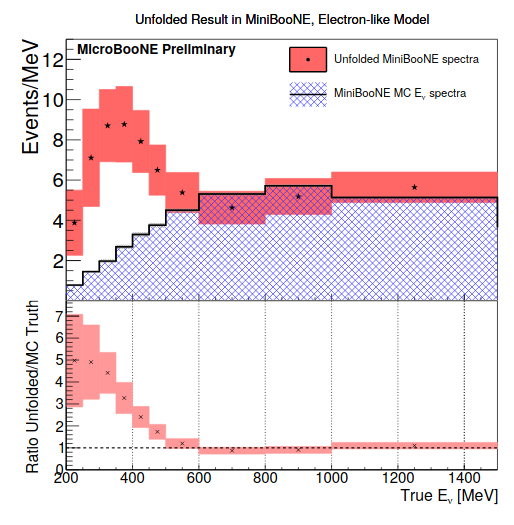
\includegraphics[width=0.45\textwidth]{introduction/unfoldedminiboone.png}
\caption{\label{fig:minibooneunfolded}MB-$\nu_e$ LEE signal model extracted from MiniBooNE's results~\cite{C2}.}
\end{center}
\end{figure}
Conceptual issues can be raised in association with the various assumptions made to generate this model. These include the strong reliance on MiniBooNE's simulation in order to unfold reconstructed to true neutrino energy, and the choice of such an unfolding procedure; for example, that it is performed as a function of $E_{\rm CCQE}$ rather than EM energy and $\theta$.
It is especially important to note that the chosen model strongly favors the interpretation of MiniBooNE events as originating from very low energies (200-400 MeV), for which achieving high sensitivity may come at the cost of omitting a robust analysis at higher energies. This is something this analysis tries to avoid by developing an inclusive and kinematically unbiased analysis. %In addition to calculating sensitivities with respect to the MB-$\nu_e$ LEE model, we explore a 3+1 sterile-neutrino oscillation model. This work, preliminary at the moment, is discussed in more detail in Section~\ref{sec:Sensitivity2Osc}.
\par Figure~\ref{fig:nuerate} shows the expected $\nu_e$ rate as a function of true neutrino energy split by final-state topology for the available MicroBooNE dataset of 10.1E20 POT. % with a 10 cm FV. 
 MB-$\nu_e$ LEE signal events are shown in orange.
\begin{figure}[H] 
\begin{center}
    \begin{subfigure}[b]{0.45\textwidth}
    \centering
    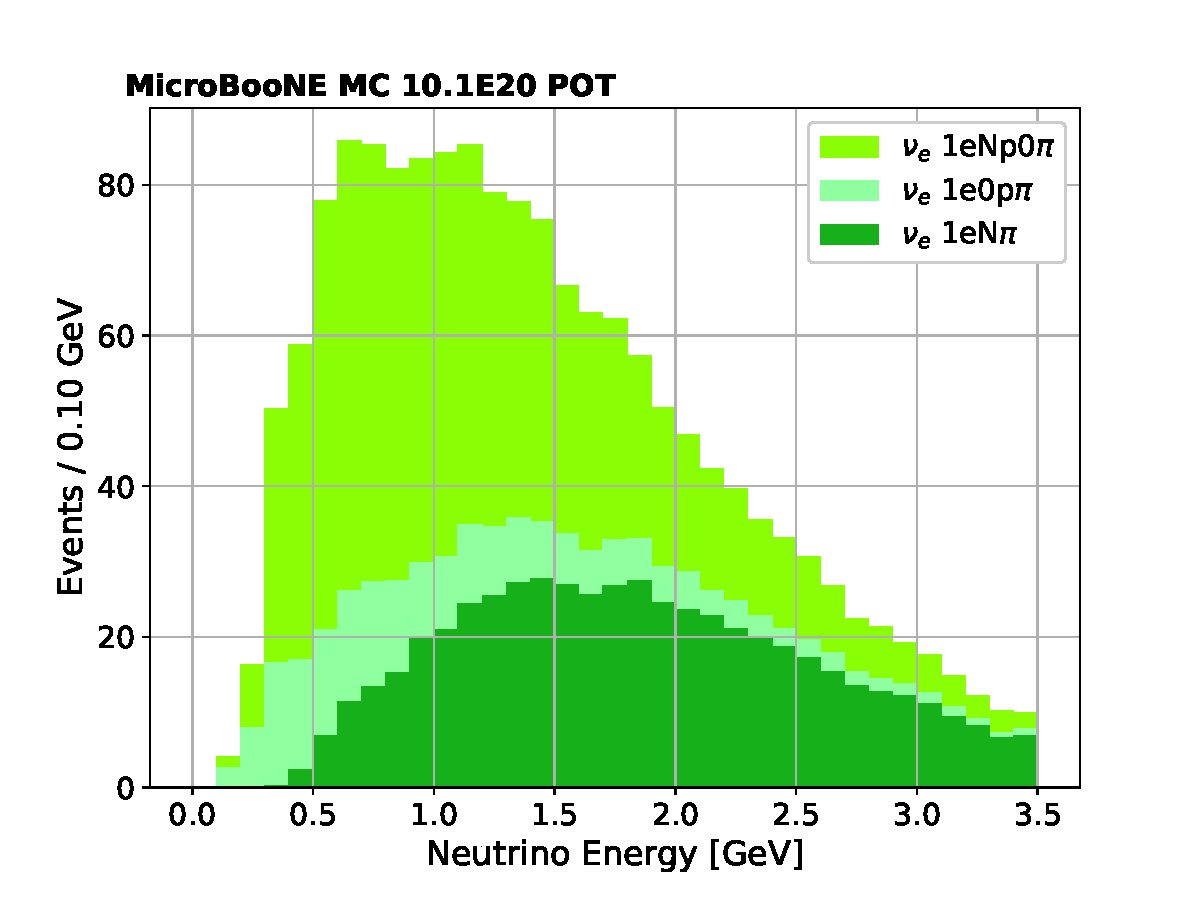
\includegraphics[width=1.00\textwidth]{introduction/nue_rate_MCC9.pdf}
    %\caption{\label{fig:nuerate:prediction}}
    \end{subfigure}
    \begin{subfigure}[b]{0.45\textwidth}
    \centering
    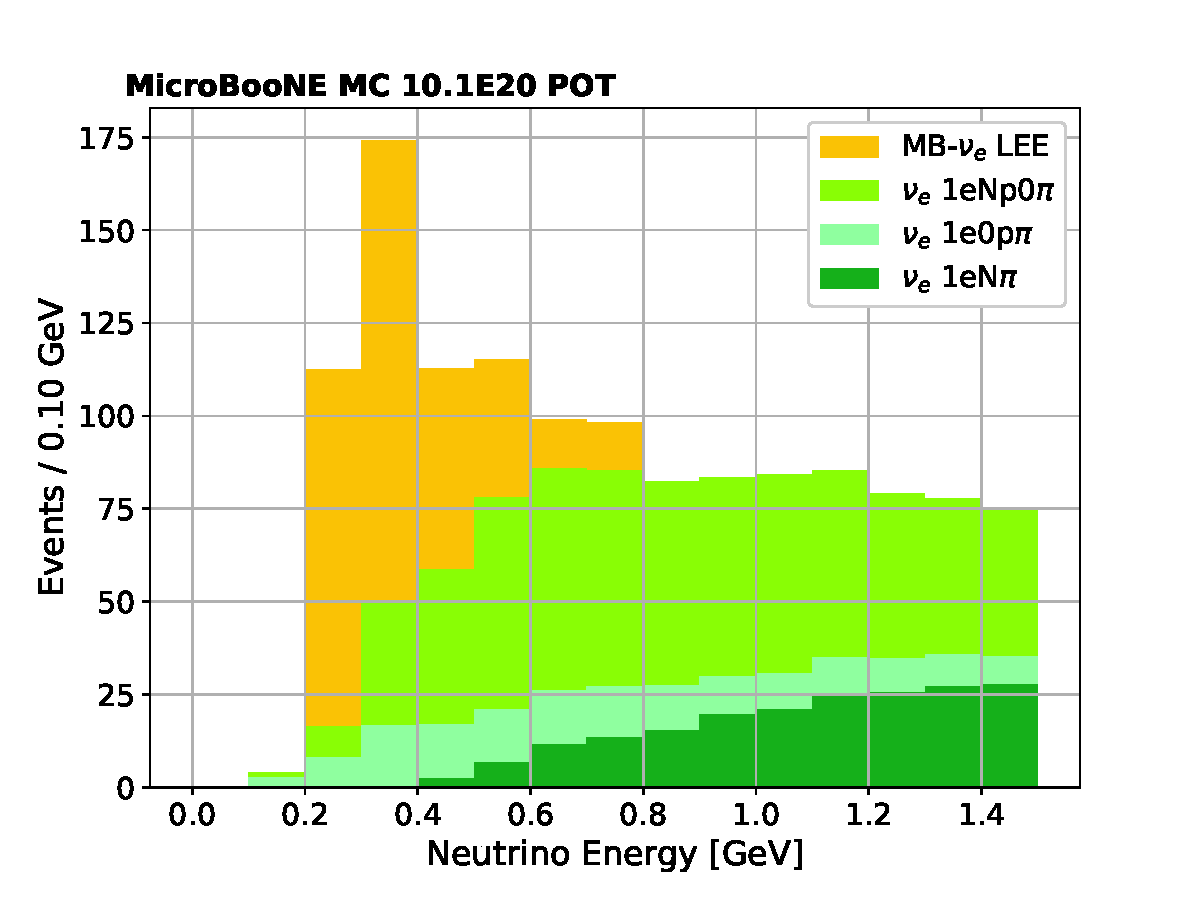
\includegraphics[width=1.00\textwidth]{introduction/nue_rate_MCC9_LEE.pdf}
    %\caption{\label{fig:nuerate:prediction:MC}}
    \end{subfigure}
\caption{\label{fig:nuerate}Expected $\nu_e$ rate in MicroBooNE for 10.1E20 POT %in a 10-cm FV 
 subdivided by event topology (1$e$N$\pi$, 1$e$N$p$0$\pi$, and 1$e$N$p$0$\pi$). The right-hand figure highlights the low energy region with the unfolded MB-$\nu_e$ LEE signal prediction in orange.}
\end{center}
\end{figure}

\subsection{Goals of the $\nu_{\mu}$ Selection}
\label{ssec:goalsofnumusel}

\par In the context of this analysis, measurements of $\nu_{\mu}$ interactions are aimed at reducing modeling uncertainties for intrinsic $\nu_e$ events and backgrounds. Event reconstruction and $\nu_e$ identification are only one of the challenges in this analysis:  in order to make statements on whether the observed $\nu_e$ rate indicates the presence of new physics, a well understood prediction of the intrinsic $\nu_e$ rate is needed. 

\par Uncertainties in the expected $\nu_e$ rate are associated with reconstruction efficiencies (detector effects), as well as modeling uncertainties in both the $\nu_e$ flux  and neutrino-argon cross-section predictions. Here, we focus on describing the strategy to deal with the latter. In the case of a single detector experiment,
flux uncertainties for $\nu_e$ calculated from the beam simulation are $\mathcal{O}$(10\%) above 800 MeV and grow to 40\% at 200 MeV. Cross-section uncertainties are also large due to the scarcity of $\nu$-Ar cross-sections measurements, especially at low energy, and due to the complex modeling of neutrino interactions on heavy targets such as argon. Combining all effects, the uncertainty on the $\nu_e$ interaction rate in the few-hundred MeV energy range in MicroBooNE is large enough to significantly hamper an analysis' sensitivity to new physics.
\par To reduce modeling uncertainties on the expected rate of $\nu_e$ interactions, data-driven constraints are required. These can be performed through measurements of $\nu_{\mu}$ interactions impacted by the same underlying modeling uncertainties. In order to constrain flux uncertainties, we rely on the fact that $\nu_e$ and $\nu_{\mu}$ intrinsic to the beam are both produced by the decay of the same parent $\pi$ and $K$ flux. Similarly, we rely on the charged-current interaction mode $\nu_{l} + Ar \rightarrow l + X$ common to both $\nu_{\mu}$ and $\nu_e$ interactions to constrain the uncertainties on the $\nu_e$ interaction modeling.

\par The richness of $\nu$-Ar interactions and of hadronic interactions in the beamline offers a number of different handles 
to constrain different uncertainties using the measurements of $\nu_{\mu}$ interactions.
As examples, measurements of CC and NC $\pi^0$ production can be used to constrain resonant interactions and thus $\pi^0$ backgrounds to the $\nu_e$ selection; measurements of high-energy $\nu_{\mu}$ interactions can help constrain the kaon flux in the beam, which contributes substantially to the production of intrinsic $\nu_e$s. Likewise, measurements of low-energy $\nu_{\mu}$s can help constrain poorly understood $\nu$-Ar interaction models in the few-hundred MeV energy regime, which is a critical requirement for this analysis. We focus our effort on the study with the largest impact to the analysis: a measurement of low-energy $\nu_{\mu}$ interactions with the goal of constraining the large uncertainties in low-energy $\nu_e$s. A detailed  description of this constraint is presented in Section~\ref{sec:sensitivity}. Preliminary work in studying high-energy $\nu_{\mu}$ events to constrain uncertainties on the kaon flux are documented in \href{https://microboone-docdb.fnal.gov/cgi-bin/private/ShowDocument?docid=31239}{DocDB 31239} but their inclusion in the analysis is left to future iterations. $\pi^0$ backgrounds are studied extensively and data-MC differences in their modeling are accounted for with the implementation of a ``tune'' described in sec.~\ref{sec:sideband:pi0}.
\par To motivate the need to study low energy $\nu_{\mu}$ interactions, we describe two important ways in which such a dataset can lead to a reduction of modeling uncertainties for $\nu_e$ interactions. Figure~\ref{fig:numuconstraint:flux} shows the flux correlation for $\nu_{\mu}$ (bottom left) and $\nu_e$ (top right) interactions obtained from MicroBooNE's adaptation of the BNB flux simulation developed by MiniBooNE~\cite{bib:fluxmcc9,bib:fluxtechnote}. Red (blue) areas show large (anti-)correlation. The top-left or bottom-right quadrants show the strength of correlations between the two flavors. For $\nu_e$ energies below 1 GeV, correlations are strongest with $\nu_{\mu}$ interactions at low energy. Figure~\ref{fig:numuconstraint:xsec} shows different cross-section predictions for $\nu_{e}$ interactions and the uncertainty on these cross-sections as assessed within GENIE-v3 and documented in~\cite{bib:1074}. Below 600 MeV, the difference in event rates for different models is significant. The large differences between these curves, particularly at low energy, indicate the strong need to constrain cross-section uncertainties with MicroBooNE data. 
\begin{figure}[ht] 
\begin{center}
    \begin{subfigure}[b]{0.42\textwidth}
    \centering
    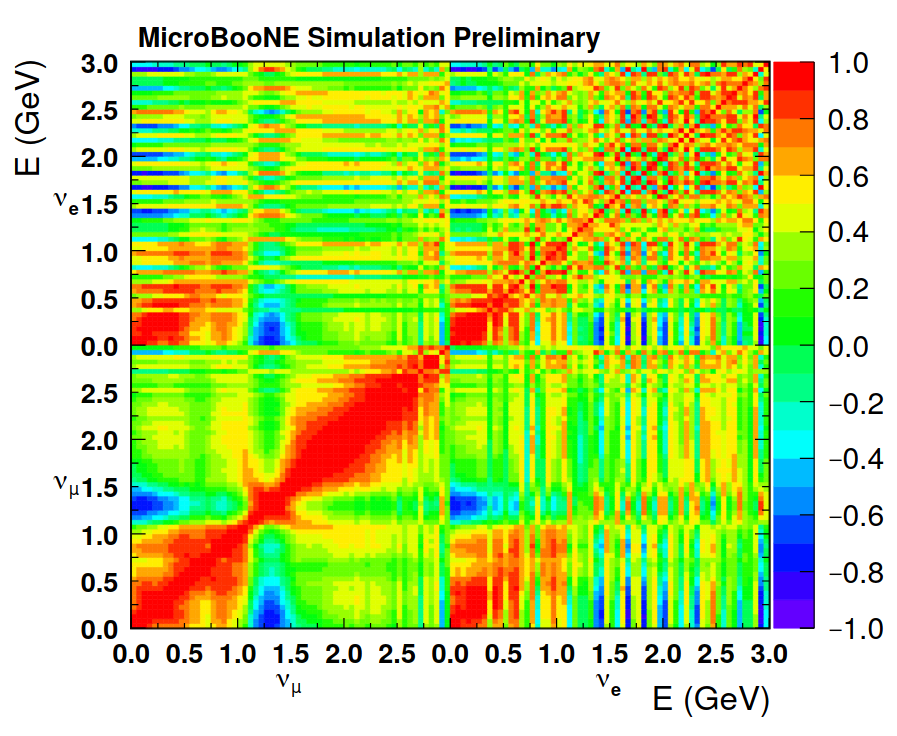
\includegraphics[width=1.00\textwidth]{introduction/fluxcorrelation.png}
    \caption{\label{fig:numuconstraint:flux} flux}
    \end{subfigure}
    \begin{subfigure}[b]{0.45\textwidth}
    \centering
    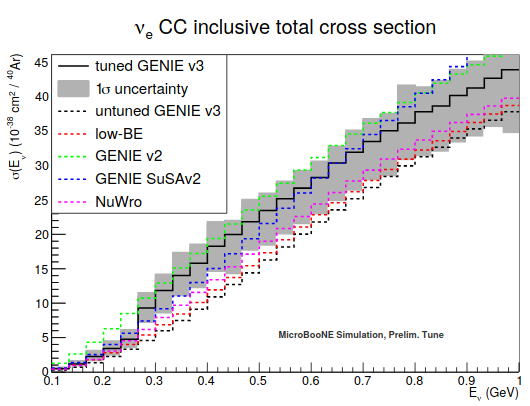
\includegraphics[width=1.00\textwidth]{introduction/lowexsec.png}
    \caption{\label{fig:numuconstraint:xsec} xsec}
    \end{subfigure}
\caption{\label{fig:numuconstraint} (a) $\nu_{\mu}-\nu_e$ flux correlation matrix at truth level from \href{https://microboone.fnal.gov/wp-content/uploads/MICROBOONE-NOTE-1031-PUB.pdf}{PUBLIC-NOTE-1031}. (b) Different cross section models and uncertainty band for $\nu_e$ CC interactions, from \href{https://microboone.fnal.gov/wp-content/uploads/MICROBOONE-NOTE-1074-PUB.pdf}{PUBLIC-NOTE-1074}~\cite{bib:1074}.}
\end{center}
\end{figure}
It should be noted that the neutrino identification work described in Section~\ref{sec:sliceID} results in a highly efficient and topology agnostic selection. A flexible selection, like this one, allows for a number of exclusive $\nu_{\mu}$ measurements and their associated constraints to be implemented in the future if the $\nu_e$ analysis needs to be more strongly constrained. 

\subsection{Systematics}
\par This section gives a brief overview of how detector and modeling uncertainties are accounted for in the analysis. The estimation of systematics is presented in section~\ref{sec:systematics}.
\par \noindent \textbf{Detector systematics}: Detector modeling in MicroBooNE has undergone significant updates in the past year, in part as a result of the large impact that detector systematics have had on 2018 analyses \cite{bib:CCpi0, bib:CCincl}. Detector effects with significant impact on the analysis can be broken up into four main categories: wire-response, space-charge, ion-recombination, and light modeling. In MCC9, the approach to detector systematics is based on studies of data-MC differences in variables relative to each effect. These observed differences are used to create detector simulation variations. These simulation variations are then used to assess the impact on the analysis' performance in measuring $\nu_e$ interactions and relative backgrounds through a uni-sim approach. The cumulative impact of detector systematics in the analysis is found to be at the 10\% level in almost all bins, and is sub-dominant compared to other sources of systematics and statistical uncertainties. The topic, including limitations in the current estimation of detector effects, is presented in detail in section~\ref{sec:detsys}.
\par \noindent \textbf{Flux, cross-section, and re-interaction modeling} Uncertainties in flux, cross-section, and particle re-interaction modeling are treated through a \emph{multi-sim} approach, where underlying parameters that are input to the model are varied in a correlated way. Flux uncertainties are taken from the MiniBooNE BNB flux simulation adapted to MicroBooNE~\cite{bib:fluxmcc9,bib:fluxtechnote}, while $\nu$ interaction uncertainties are handled within the \texttt{GENIE} reweighting package, as described in~\cite{bib:geniesupportnote}. Particle re-interaction uncertainties (subdominant, at the 1\% level) are included following the treatment oulined in~\href{https://microboone-docdb.fnal.gov/cgi-bin/private/ShowDocument?docid=31919}{DocDB 31919}. The assessment of flux, cross-section, and re-interaction uncertainties and their impact on the analysis are described in sections~\cref{sec:systematics:flux},~\cref{sec:systematics:xsec}, and~\cref{sec:systematics:reint} respectively.

Figure~\ref{fig:systsummaryintro} summarizes the impact of systematic uncertainties on the three channels used in the LEE sensitivity estimation. For $\nu_e$ channels, the total uncertainty before and after constraint are shown in dotted and solid black lines respectively. It is important to note that, while not represented in the plot, statistical errors dominate the uncertainty in the $\nu_e$ selections, while are negligible in the $\nu_{\mu}$ channel.

\begin{figure}[H] 
\begin{center}
    \begin{subfigure}[b]{0.32\textwidth}
    \centering
    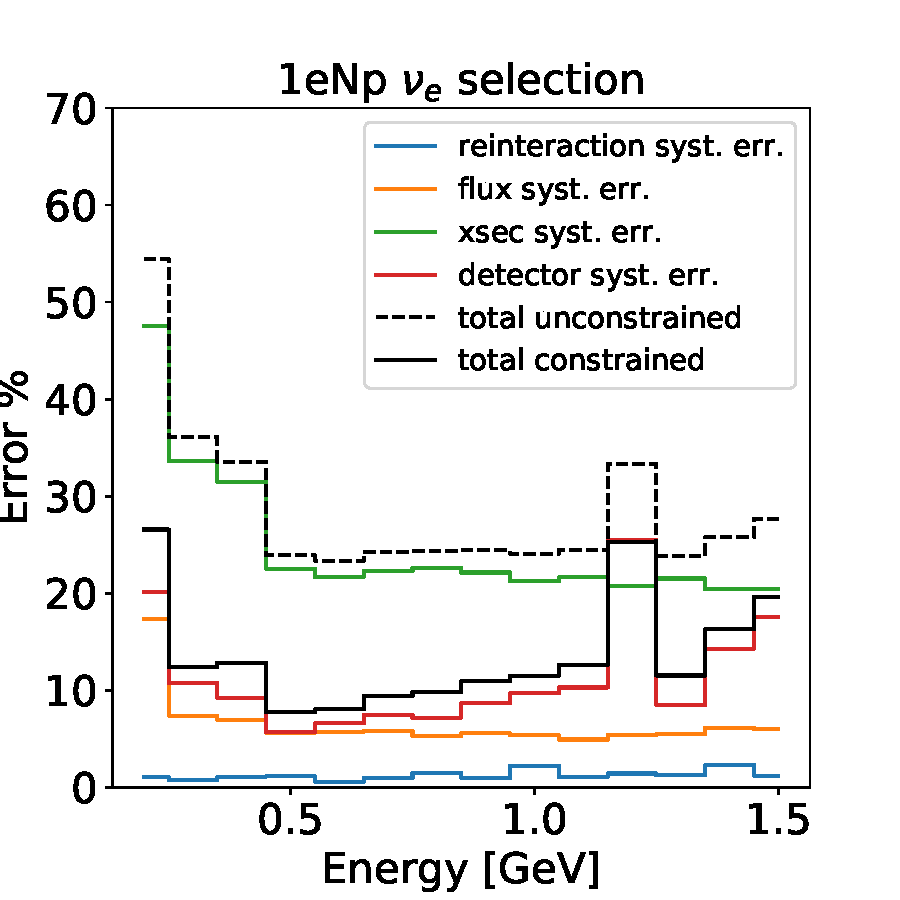
\includegraphics[width=1.00\textwidth]{Systematics/1eNp_syst_summary.pdf}
    \caption{\label{fig:systsummary:np}\npsel}
    \end{subfigure}
    \begin{subfigure}[b]{0.32\textwidth}
    \centering
    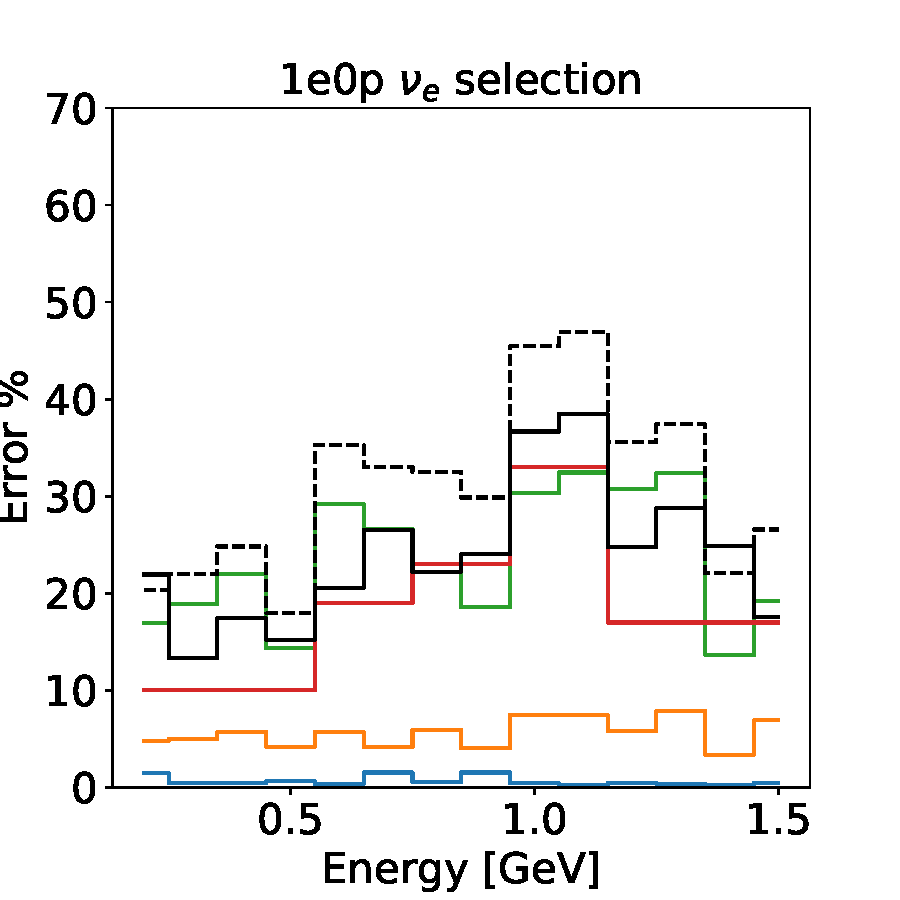
\includegraphics[width=1.00\textwidth]{Systematics/1e0p_syst_summary.pdf}
    \caption{\label{fig:systsummary:zp}\zpsel}
    \end{subfigure}
    \begin{subfigure}[b]{0.32\textwidth}
    \centering
    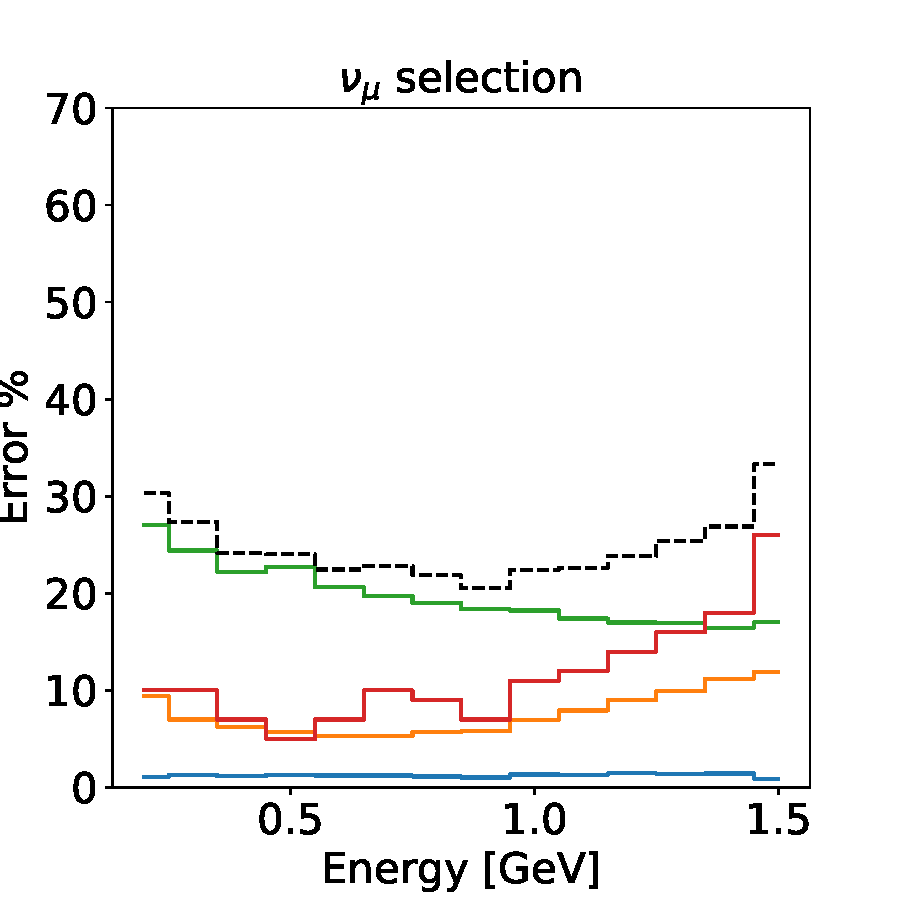
\includegraphics[width=1.00\textwidth]{Systematics/numu_syst_summary.pdf}
    \caption{\label{fig:systsummary:numu}\numu}
    \end{subfigure}
\caption{\label{fig:systsummaryintro}Summary of systematic errors on the analysis in the three selections used for the LEE sensitivity estimation.}
\end{center}
\end{figure}


\subsection{Sensitivity Estimation}
Given a measurement of the spectrum of reconstructed $\nu$ energy in the \npsel and \zpsel event distributions, the hypothesis in which the observed spectrum is entirely due to the Standard Model (SM), $H_0$, is tested against an alternative hypothesis $H_1$.
The alternative hypothesis $H_1$ consists of all background and intrinsic $\nu_e$ events (i.e. the SM hypothesis), plus the LEE unfolded signal from MiniBooNE (MB-$\nu_e$ LEE).
In this analysis a simple hypothesis test is performed to test compatibility of the data with $H_0$ vs. $H_1$, and no signal strength is extracted.

A test statistic is chosen in order to condensate all information of the observables in one number.
Through toy experiments, the expected distributions of the test statistic under the two hypotheses is calculated; the separation power is computed by taking the median p-value with respect to $H_0$ under the assumption that $H_1$ is true. This is the discovery sensitivity, i.e. the sensitivity to reject $H_0$ when $H_1$ is true.
%We studied the sensitivity in different cases. First, we describe in detail the sensitivity calculation considering only statistical uncertainties. Given the current efficiency for low-energy $\nu_e$ interactions, the impact of statistical uncertainties plays a large role in determining the analysis' ultimate sensitivity. We also include systematic uncertainties using the covariance matrix formalism and the SBNfit package, as described in section \ref{subsec:sensitivity_syst_uncertainty}.
The full sensitivity calculation takes all observed spectra from the \npsel, \zpsel, and \numu selections and analyzes them simultaneously using a single covariance matrix to constrain the systematic uncertainties and thus increase the sensitivity.

\subsection{Results}
\label{sec:introduction:conclusions}
\par The work presented in this note has matured into a robust and comprehensive analysis, with strong tools which are able to leverage the calorimetric and topological imaging of the LArTPC technology to identify in a kinematically agnostic selection $\nu_e$ interactions in MicroBooNE's BNB dataset. The analysis, as it stands, is able to make interesting conclusions about the $\nu_e$ content of the BNB flux, with the primary limitation to the power of these conclusions driven by the low selection efficiency at low energy.
\par Multiple selections have been developed as part of this analysis, all showing generally good data-simulation agreement. Validations of the analysis through data/MC comparisons have been performed in several sideband regions and are summarized in figures~\ref{fig:datamccomparisons1},~\ref{fig:datamccomparisons2}, and~\ref{fig:datamccomparisons3}. These figures showcase the broad data validations performed by this analysis over different samples, energy regimes, and beams. Data-MC comparisons in all variables used in the analysis, at relevant stages of a selection are showed in the numerous appendices of this Tech Note. Most data-MC comparisons provided in this note are now derived from far-sideband samples, described in detail in Sec.~\ref{sec:sidebands}. %The analysis team has devised and a procedure for reaching a final box-opening which relies on producing successively more sensitive data-MC comparisons of distributions relevant to the analysis, starting with the $\pi^0$ and $\nu_{\mu}$ sideband and constraint channels, and moving to distributions relevant to the $\nu_e$ channel. This procedure, outlined in \href{https://microboone-docdb.fnal.gov/cgi-bin/private/ShowDocument?docid=28527}{DocDB 28527} is being developed in accordance to the guidelines of the OSC group presented in \href{https://microboone-docdb.fnal.gov/cgi-bin/private/ShowDocument?docid=29203}{DocDB 29203}.

\begin{figure}[H] 
\begin{center}
    \begin{subfigure}[b]{0.3\textwidth}
    \centering
    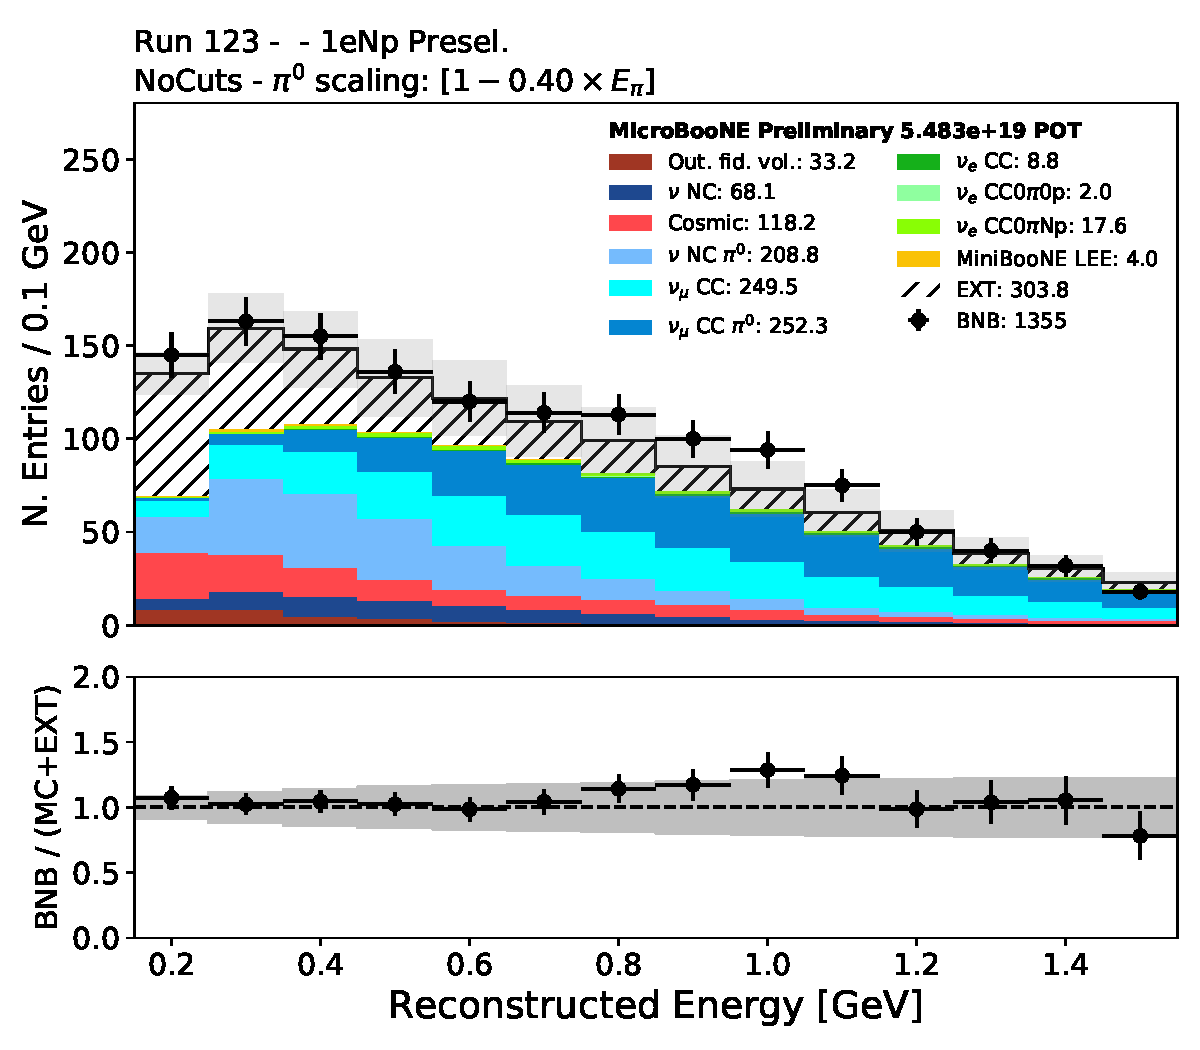
\includegraphics[width=1.00\textwidth]{1eNp/reco_e_presel.pdf}
    \caption{\label{fig:datamccomparisons:nuepresel} \npsel pre-selection for Run  1}
    \end{subfigure}
    \begin{subfigure}[b]{0.3\textwidth}
    \centering
    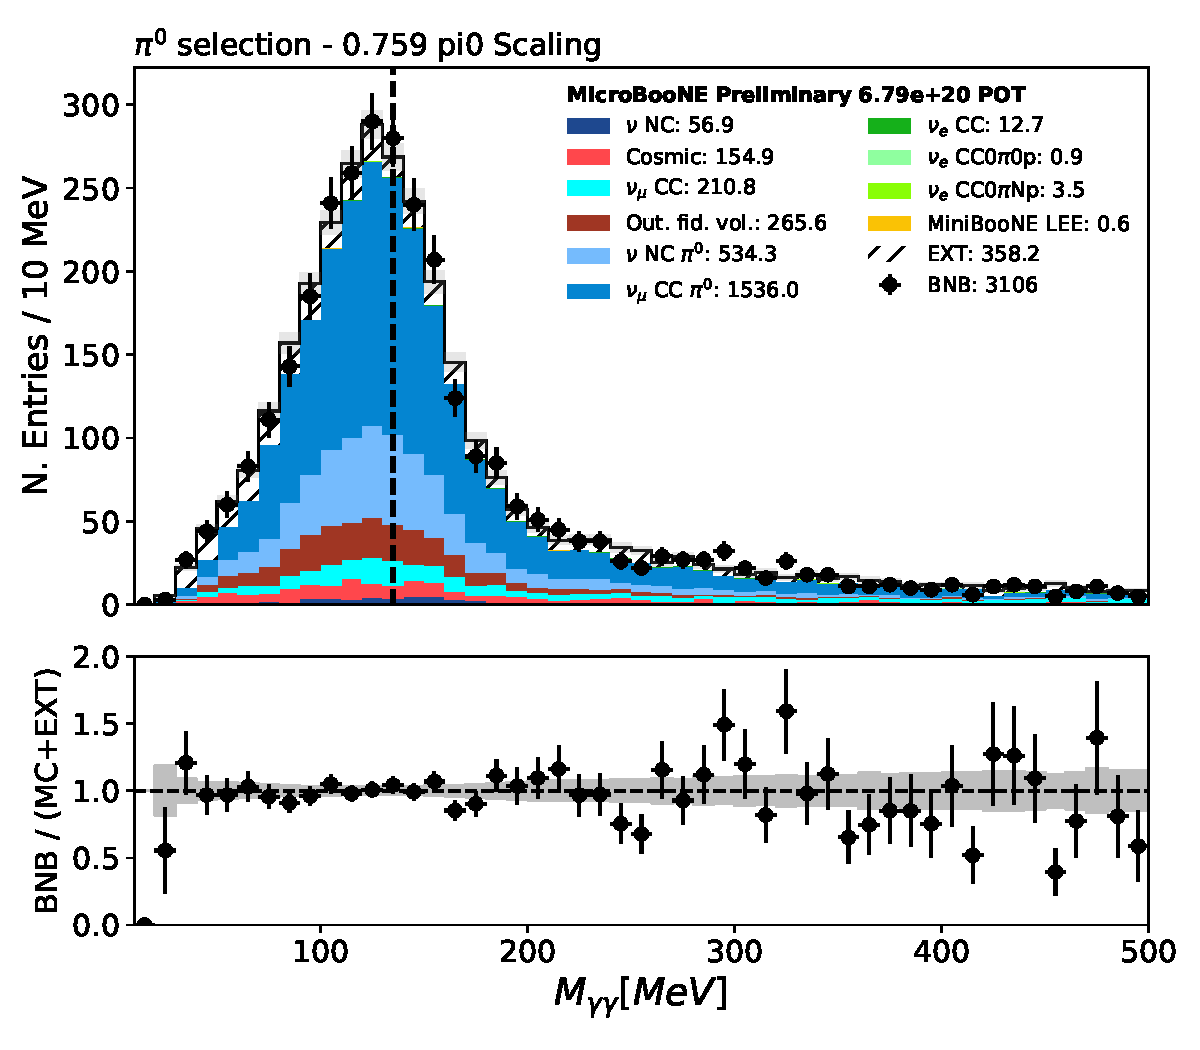
\includegraphics[width=1.00\textwidth]{pi0/calorimetry/pi0_mass_Y_corr_run123.pdf}
    \caption{\label{fig:datamccomparisons:numu} $\pi^0$s area-normalized}
    \end{subfigure}
    \begin{subfigure}[b]{0.3\textwidth}
    \centering
    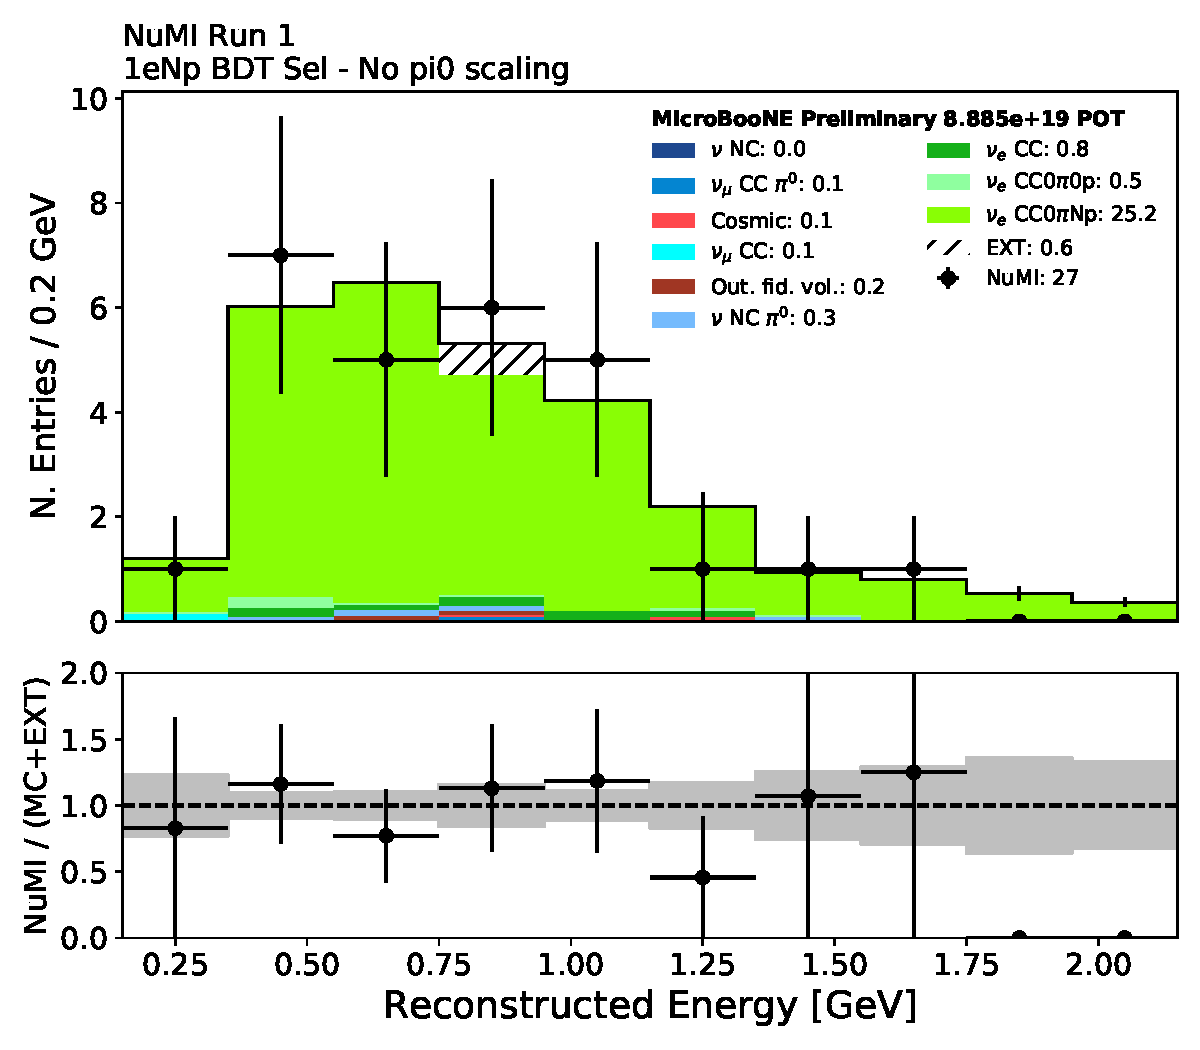
\includegraphics[width=1.00\textwidth]{Sidebands/Figures/NuMI/1eNp/BDTSel/reco_e.pdf}
    \caption{\label{fig:datamccomparisons:pi0} NuMI \npsel}
    \end{subfigure}
\caption{\label{fig:datamccomparisons1} data-mc comparisons from various sidebands.}
\end{center}
\end{figure}

\begin{figure}[H] 
\begin{center}
    \begin{subfigure}[b]{0.3\textwidth}
    \centering
    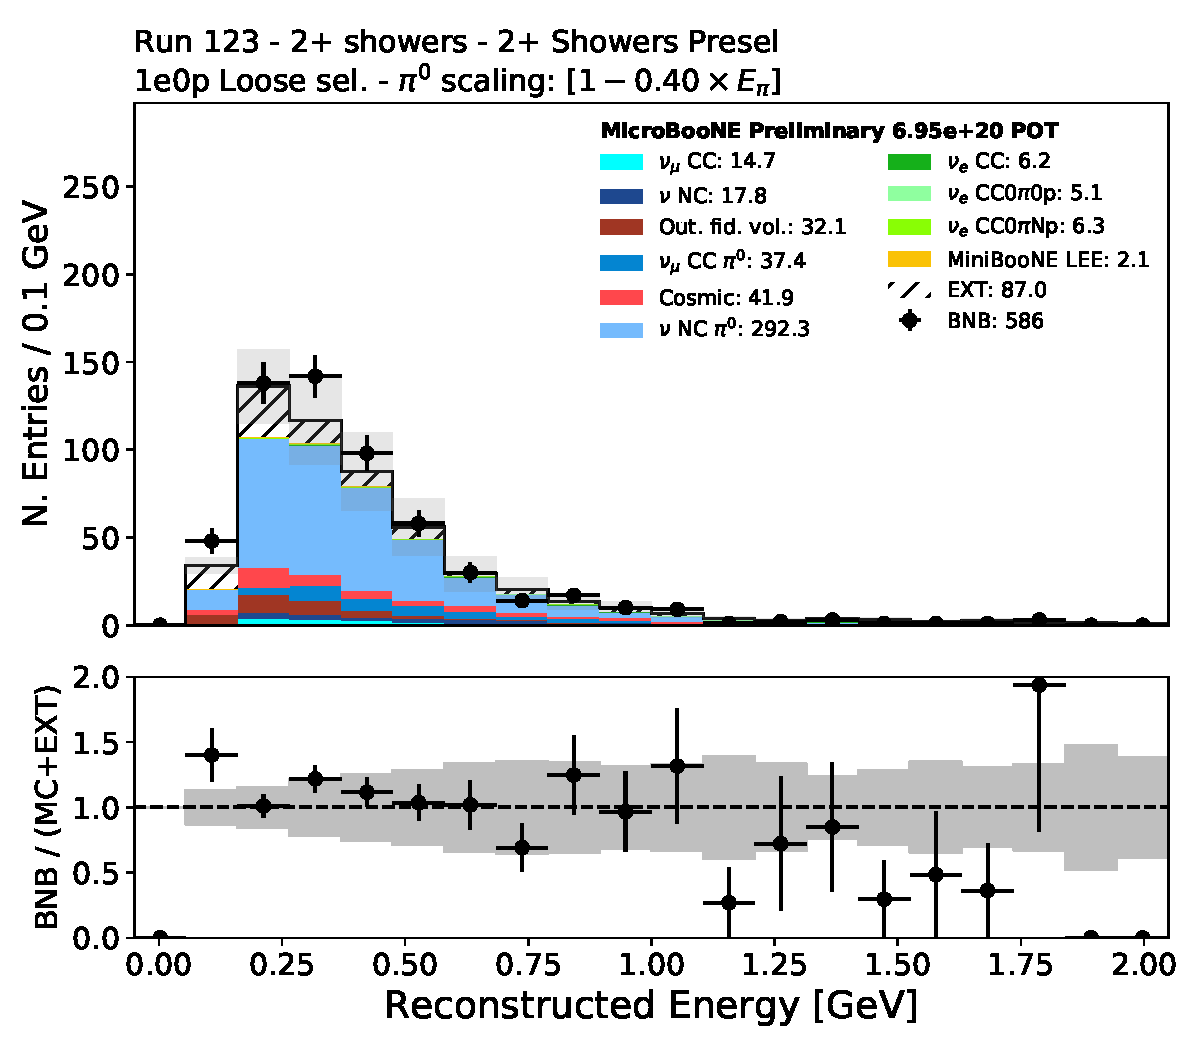
\includegraphics[width=1.00\textwidth]{Sidebands/Figures/TwoShr_1e0pSel_newSamples/reco_e_loose.pdf}
    \caption{\label{fig:datamccomparisons:nuepresel} 2+ shower \npsel}
    \end{subfigure}
    \begin{subfigure}[b]{0.3\textwidth}
    \centering
    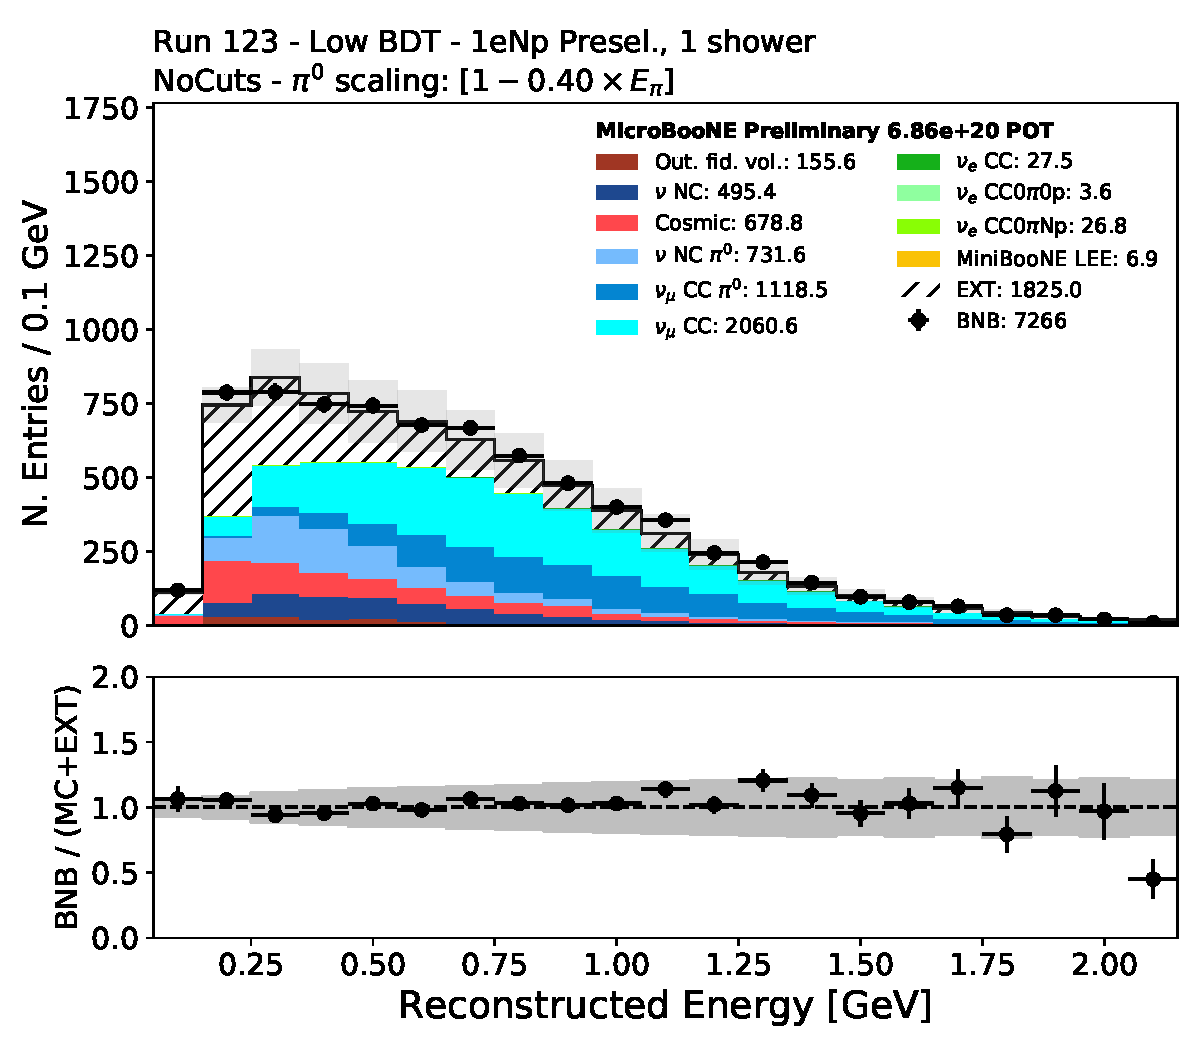
\includegraphics[width=1.00\textwidth]{Sidebands/Figures/1eNp/LPID_NPOneShr_None_pi0e40/reco_e.pdf}
    \caption{\label{fig:datamccomparisons:numu} low-PID \npsel}
    \end{subfigure}
    \begin{subfigure}[b]{0.3\textwidth}
    \centering
    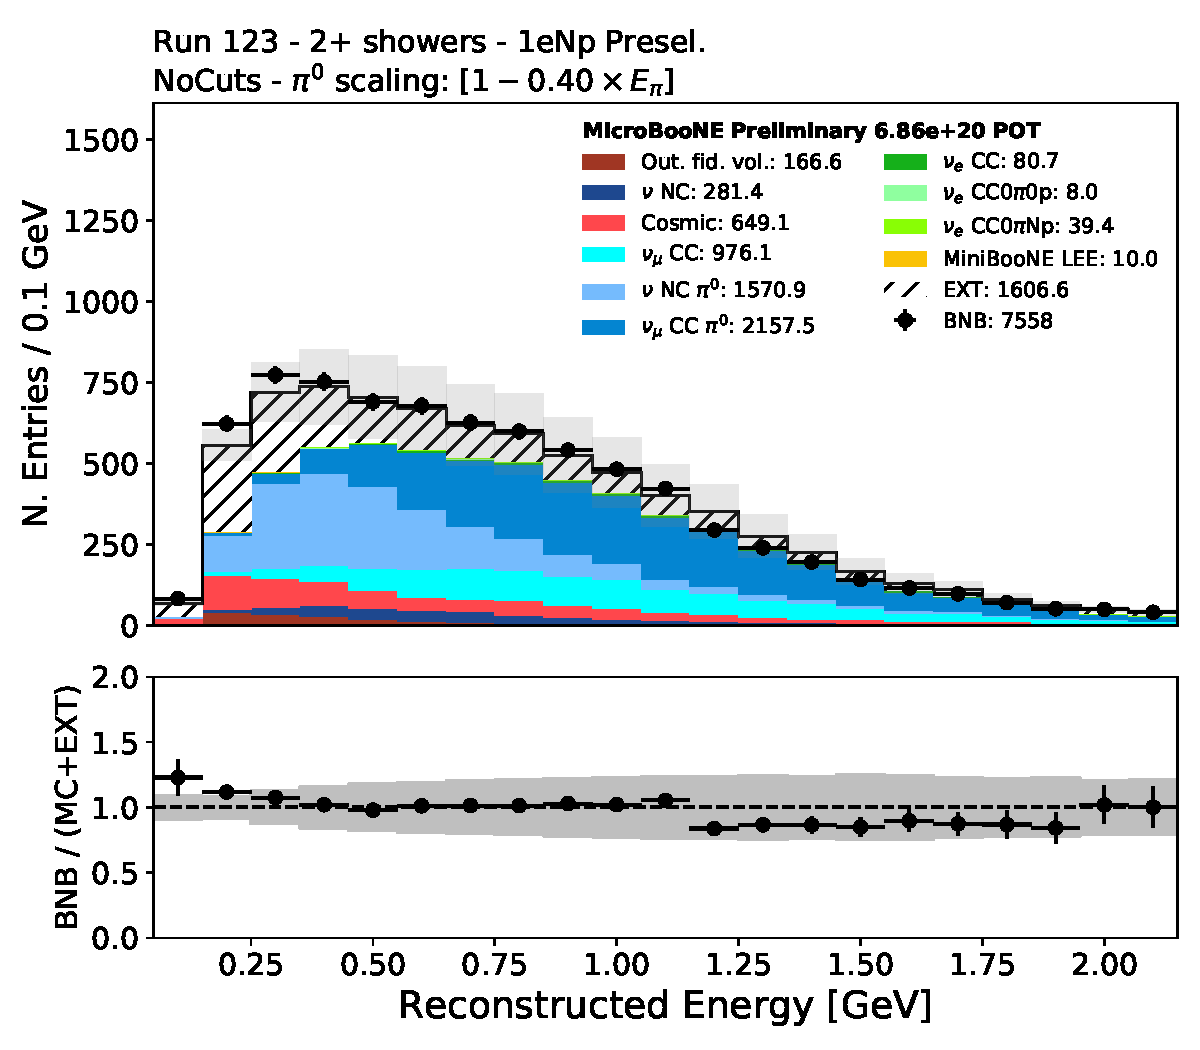
\includegraphics[width=1.00\textwidth]{Sidebands/Figures/1eNp/TwoShower/TwoPShr_NP_None_pi0e040/reco_e.pdf}
    \caption{\label{fig:datamccomparisons:pi0} 2+ shower \zpsel}
    \end{subfigure}
\caption{\label{fig:datamccomparisons2} data-mc comparisons from various sidebands.}
\end{center}
\end{figure}

\begin{figure}[H] 
\begin{center}
    \begin{subfigure}[b]{0.3\textwidth}
    \centering
    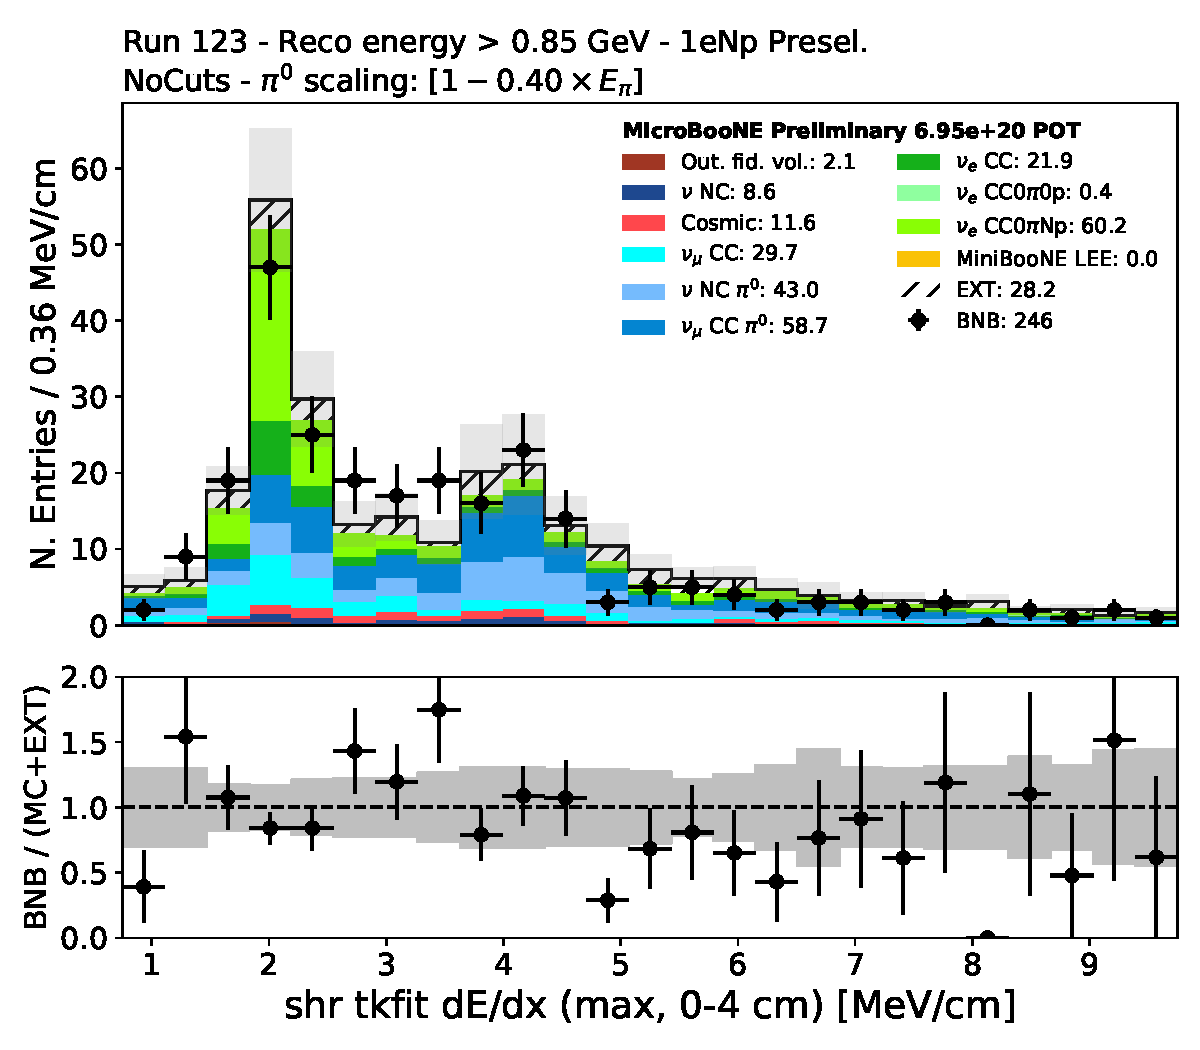
\includegraphics[width=1.00\textwidth]{egamma/shr_tkfit_dedx_max_run123_trkpid_lt_m01_tkshdistance_10cm.pdf}
    \caption{\label{fig:datamccomparisons:nuepresel} \zpsel \dedx}
    \end{subfigure}
    \begin{subfigure}[b]{0.3\textwidth}
    \centering
    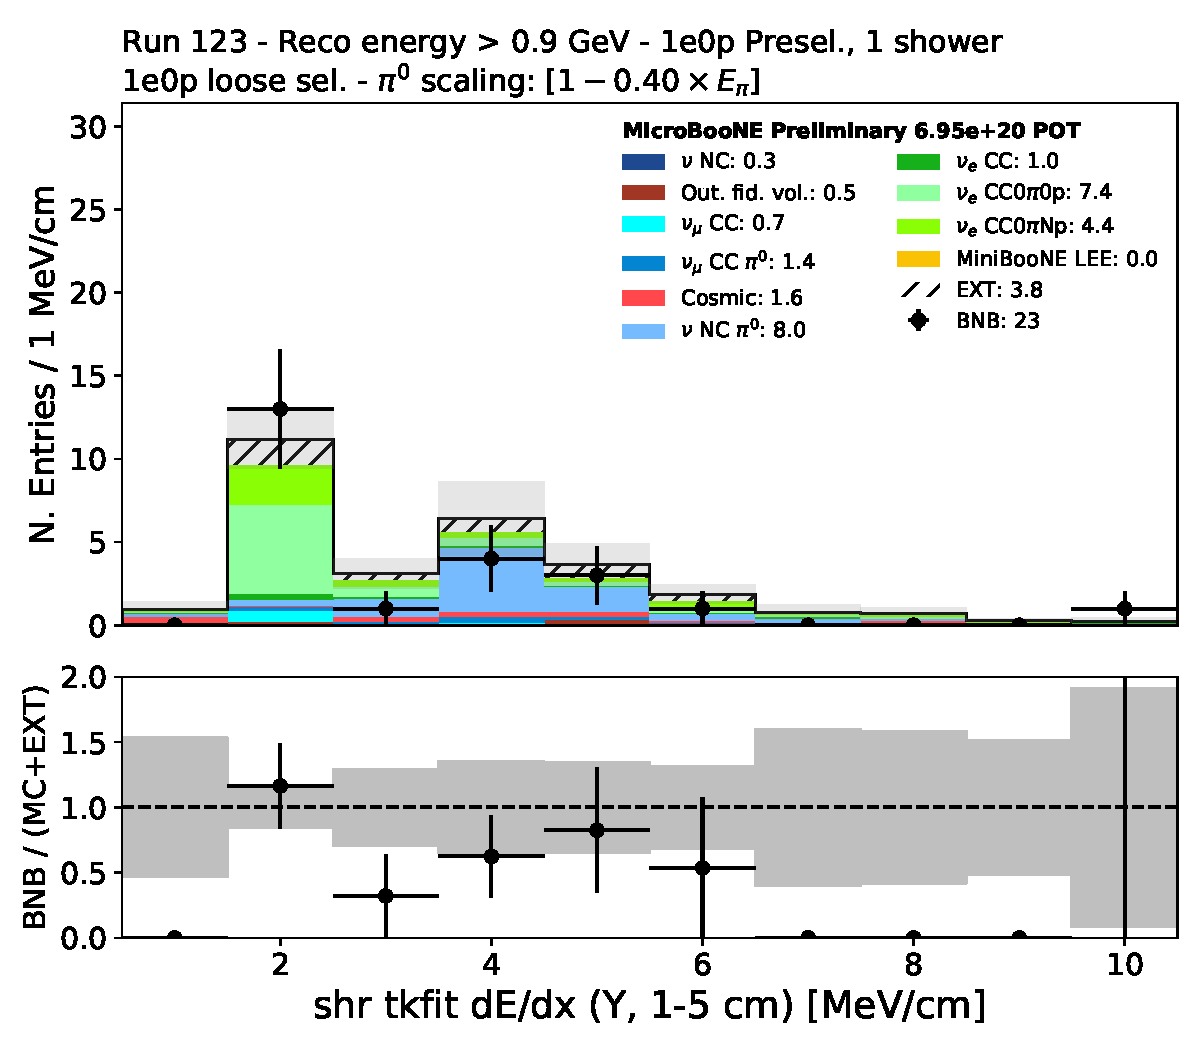
\includegraphics[width=1.00\textwidth]{1e0p/High_E_Sideband/loose_selection/shr_tkfit_gap10_dedx_Y.pdf}
    \caption{\label{fig:datamccomparisons:numu} \npsel \dedx}
    \end{subfigure}
    \begin{subfigure}[b]{0.17\textwidth}
    \centering
    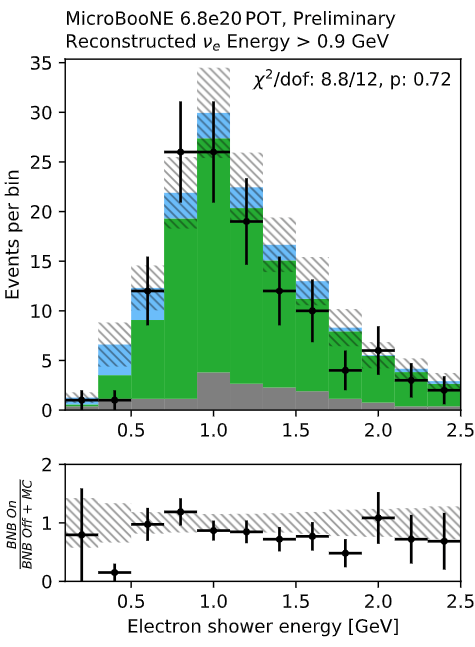
\includegraphics[width=1.00\textwidth]{introduction/inclHE.png}
    \caption{\label{fig:datamccomparisons:pi0} \nue inclusive HE}
    \end{subfigure}
\caption{\label{fig:datamccomparisons3} data-mc comparisons from various sidebands}
\end{center}
\end{figure}

\par The three selections employed in the sensitivity calculation are shown in figure~\ref{fig:intro:nueselections}, which includes the  \npsel (figure~\ref{fig:intro:nueselections:1eNp}) and \zpsel selection (figure~\ref{fig:intro:nueselections:1e0p}) with data-points for the energy bin accessible through the far-energy sidebands. Figure ~\ref{fig:intro:nueselections:numu} shows the full \numu selection used as a constraint. %The two exclusive \npsel and \zpsel selections provide sensitivity to new physics in the $\nu_e$ channel, focusing at low-energy. 
\par The \npsel channel achieves a $7-15$\% efficiency with an energy-dependent 60-90\%  purity, leading to $\mathcal{O}$(10) expected MB-$\nu_e$ LEE signal events and $70$ intrinsic $\nu_e$ events for the full Run $1-3$ data set.% The final reconstructed energy distribution for the BDT selection is shown in figure~\ref{fig:intro:nueselections}.  
\par The \zpsel channel obtains a purity of 50\%. This channel, in addition to providing a valuable constraint of detector and modeling effects which can cause migration from the \npsel to the \zpsel channel, also adds to the performance of the analysis because it is treated on equal footing as the \npsel in the sensitivity calculation.
\par Finally, the inclusive channel provides the analysis a tool with which to study the modeling of $\nu_e$ interactions, especially at higher energies, and provides a first validation even with the small data set currently available.

\begin{figure}[ht] 
\begin{center}
    \begin{subfigure}[b]{0.3\textwidth}
    \centering
    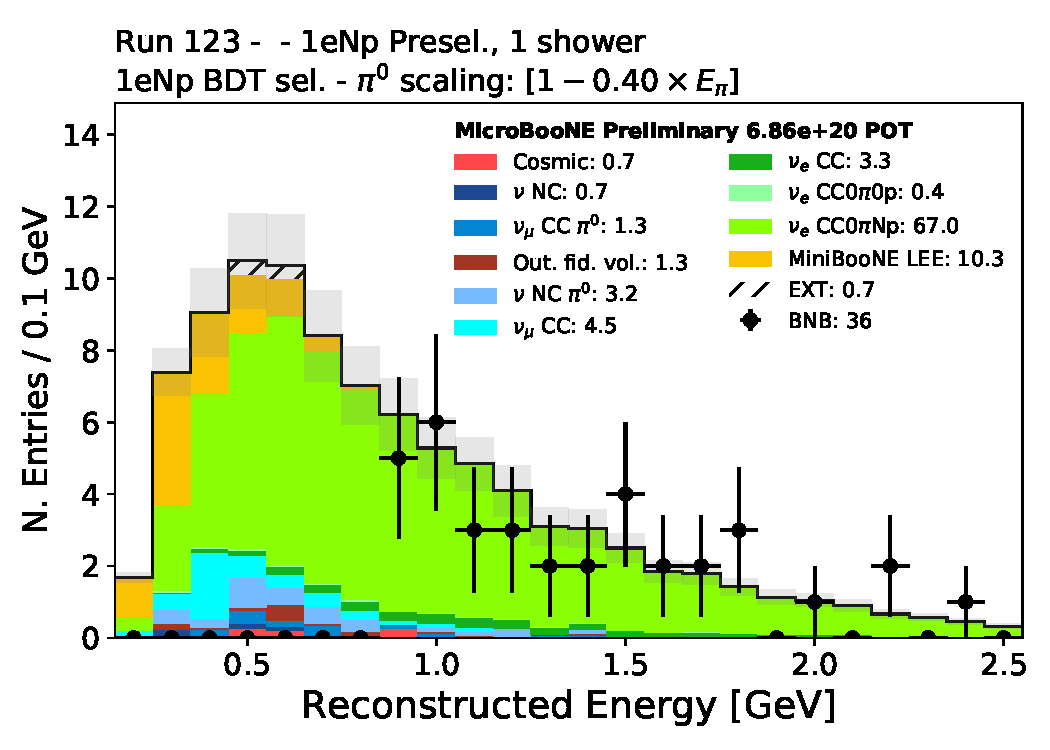
\includegraphics[width=1.00\textwidth]{Sidebands/Figures/1eNp/HighEnergy/reco_e.pdf}
    \caption{\label{fig:intro:nueselections:1eNp}\npsel}
    \end{subfigure}
    \begin{subfigure}[b]{0.3\textwidth}
    \centering
    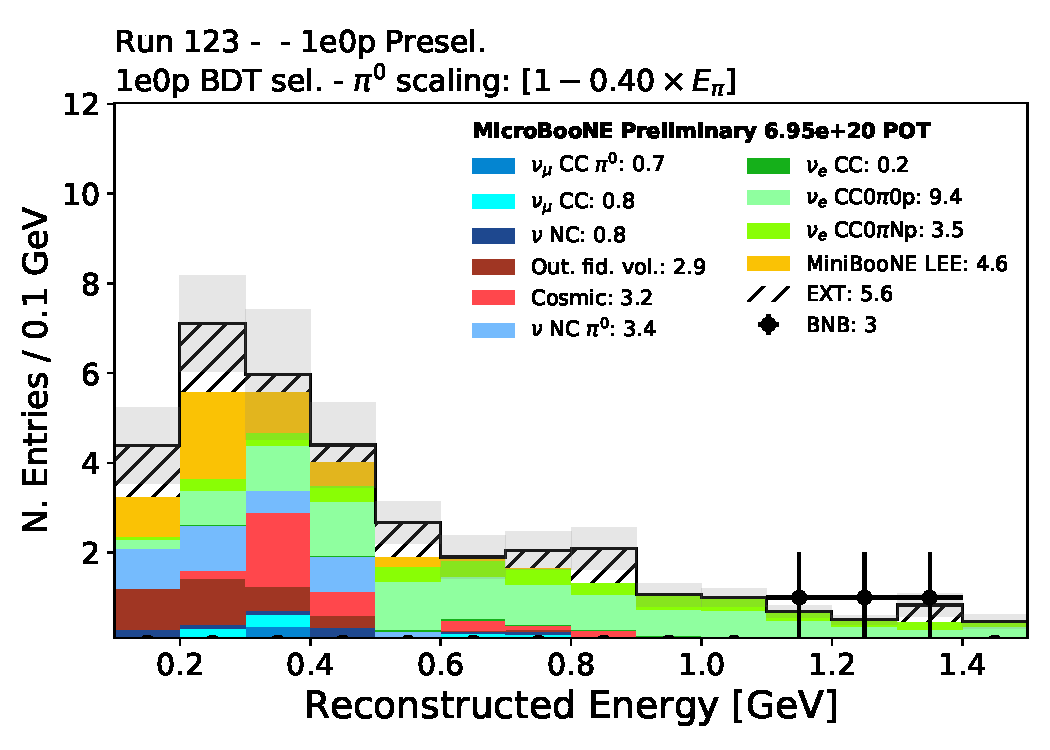
\includegraphics[width=1.00\textwidth]{introduction/reco_e_1e0p_08052020.pdf}
    \caption{\label{fig:intro:nueselections:1e0p}\zpsel}
    \end{subfigure}
    \begin{subfigure}[b]{0.28\textwidth}
    \centering
    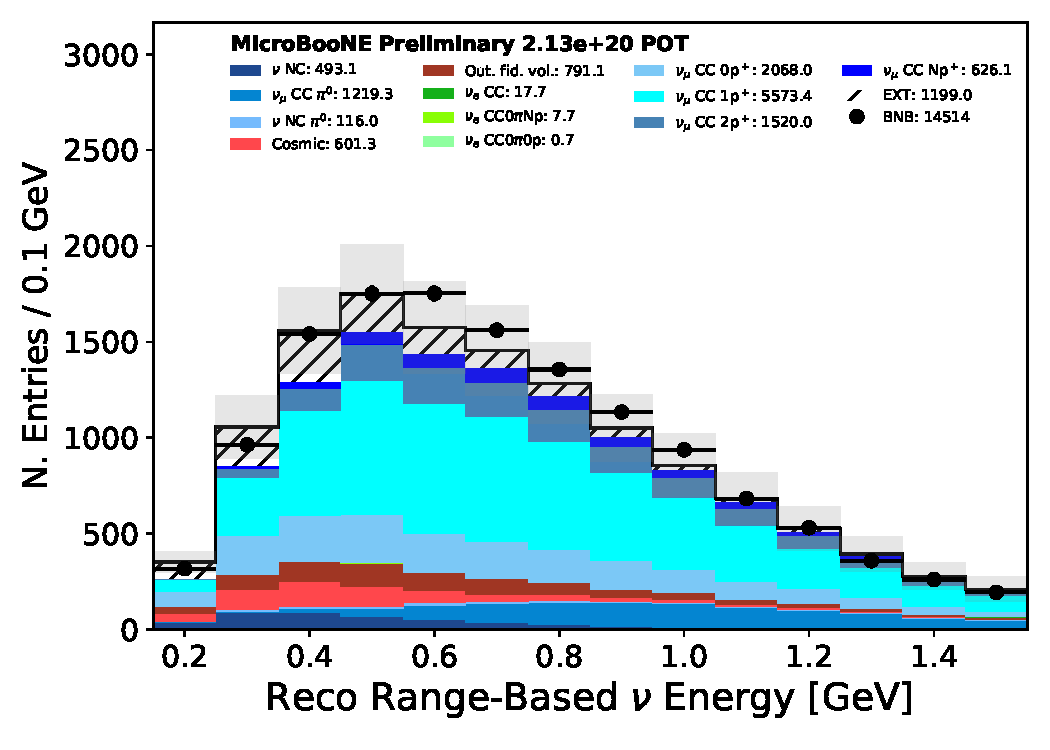
\includegraphics[width=1.00\textwidth]{NuMuCCsel/Images/Ryan/fullselection_run3_fullsystematics/reco_nu_e_range_v_08052020_fullsel_samples_noratio_event_category.pdf}
    \caption{\label{fig:intro:nueselections:numu} $\nu_{\mu}$}
    \end{subfigure}
\caption{\label{fig:intro:nueselections} Final spectra of the \npsel, \zpsel, and \numu selections in reconstructed neutrino energy provided as input to SBNFit. Data-points are shown for \nue events in the far-sideband (above 0.85 and 0.9 GeV for the \npsel and \zpsel respectively) and for the full spectrum for \numu events.}
\end{center}
\end{figure}


\par The high-quality inclusive contained $\nu_{\mu}$ selection (section~\ref{sec:nueselection:inclusive}) shows good data-simulation agreement in both Run 1 and Run 3 and provides the input for the $\nu_{\mu}$ constraint which has the primary goal of reducing systematic uncertainties for low-energy $\nu_e$s. An initial estimation of the impact of the $\nu_{\mu}$ constraint shows a 50\% reduction in modeling uncertainties. Additionally, an inclusive $\nu_{\mu}$ selection provides a valuable starting point for many possible final-state measurements which may become necessary to further validate the analysis. 
\par The current version of the analysis, which includes the use of the SBNFit framework and accounts for flux, cross-section, and re-interaction uncertainties (constrained through the $\nu_{\mu}$ channel) as well as detector uncertainties leads to a 2.3$\sigma$ median sensitivity to exclude the SM in favor of the LEE hypothesis with the full Run 1$-$3 6.95E20 POT data set. 
\begin{figure}[H]
    \begin{center}
    \begin{subfigure}{0.55\textwidth}
    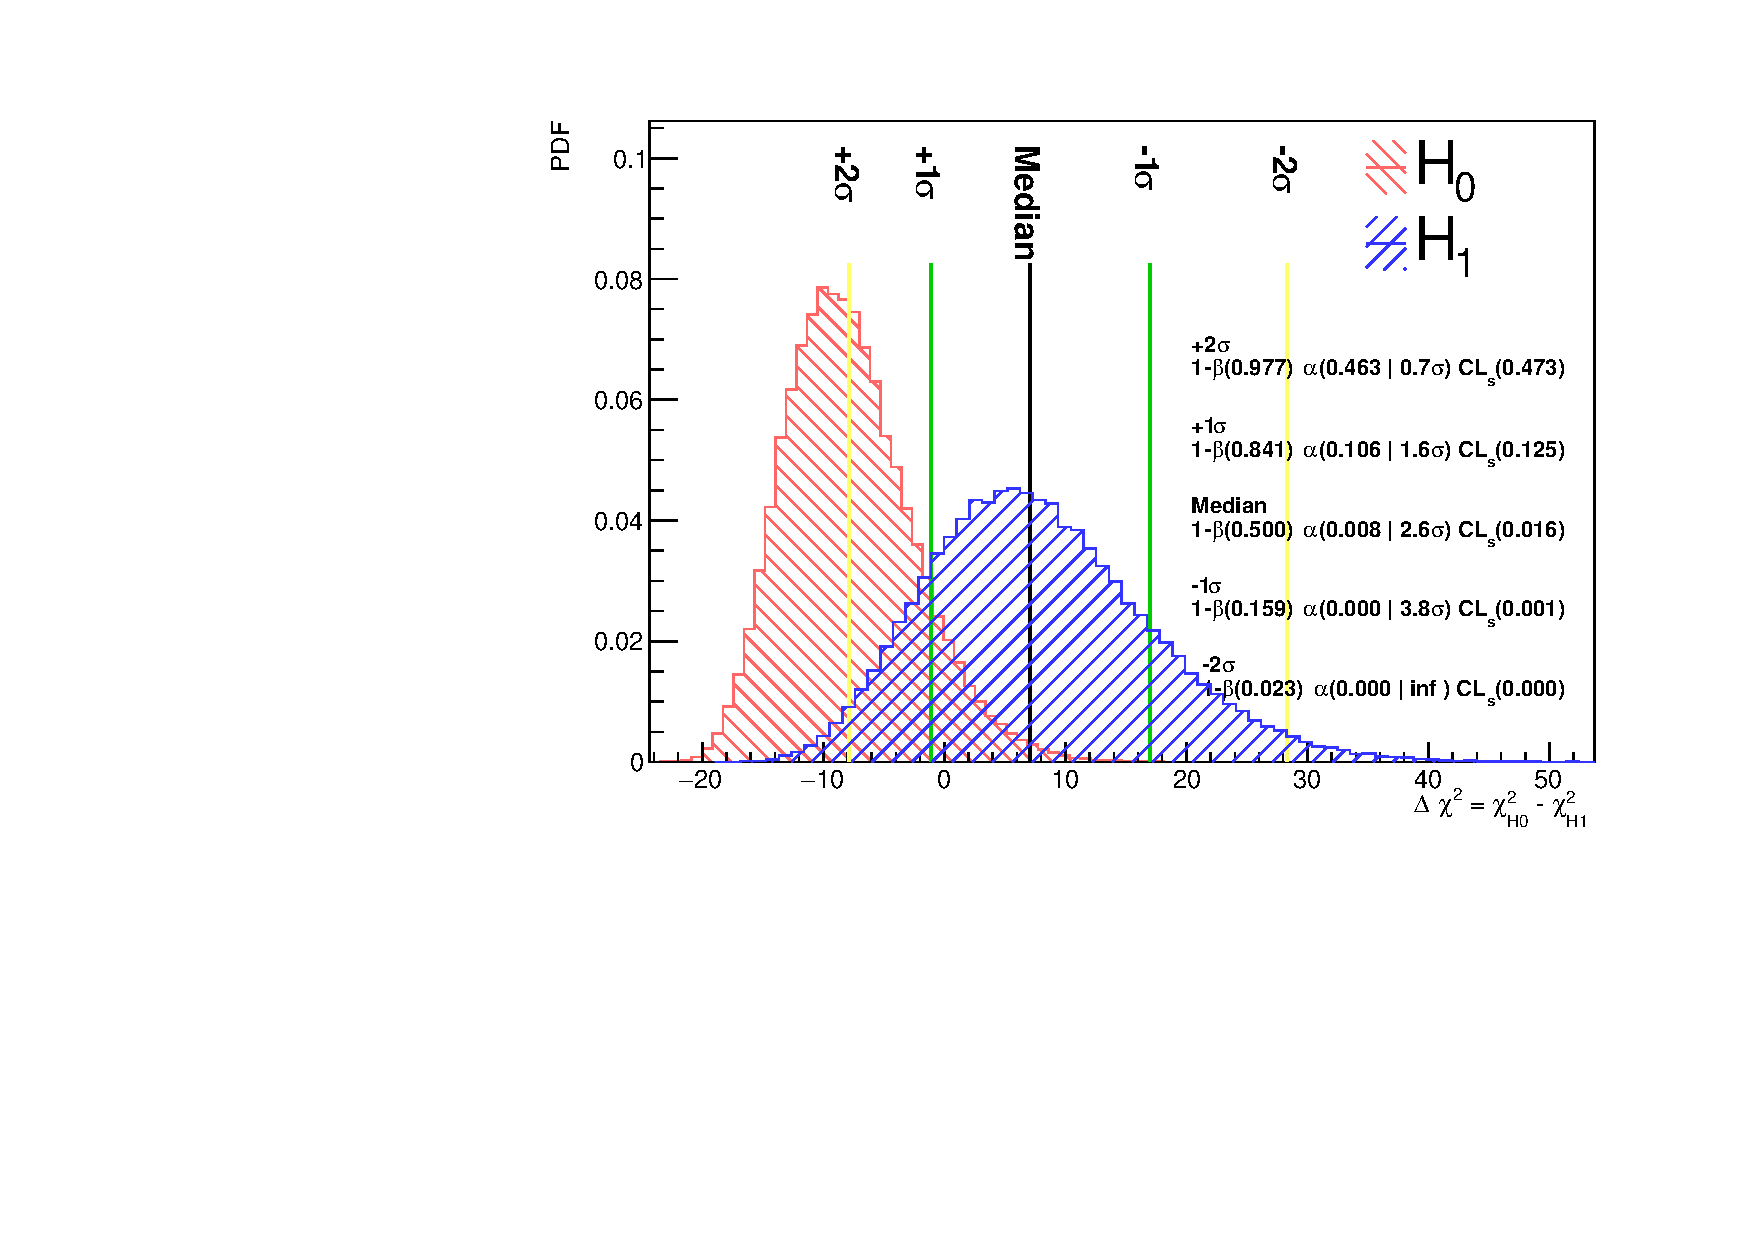
\includegraphics[width=1.00\textwidth]{Sensitivity/BDT_higheff/SBNfit_Cls_nue_1e0p_numu_reco_e_H1_newBDT_higheff_noCCMEC_constrained_detsys.pdf}
    \label{fig:sensitivity_bdt_loose_const:intro}
    %\caption{Loose BDT selection}
    \end{subfigure}
    \caption{Final discovery sensitivity to the LEE unfolded signal of the \npsel selection with the constrained systematics.}
    \end{center}
\end{figure}

\begin{table}[H]
\centering
\setlength{\tabcolsep}{10pt}
\renewcommand{\arraystretch}{1.25}
 \begin{tabular}{| c | c | c | m{2.3 cm} | c | c | c |} 
 \hline
 POT & LEE events & \nue events & scenario & stat. $\sigma$  & stat+syst. $\sigma$ & constrained $\sigma$ \\
 \hline
\multirow{2}{*}{$6.95E20$} &  \multirow{2}{*}{14.97} & \multirow{2}{*}{74.97} & ruling out SM if LEE is true & $2.5$ & $1.9$ & $2.3$ \\
 &  &  & ruling out LEE if SM is true & $2.2$ & $1.9$ & $2.2$ \\
\multirow{2}{*}{$12.5E20$} & \multirow{2}{*}{26.91} & \multirow{2}{*}{134.85} & ruling out SM if LEE is true & $3.3$ & $2.3$ & $3.0$ \\
 &  &  & ruling out LEE if SM is true &$3.0$ & $2.5$ & $2.9$ \\
 \hline
 \end{tabular}
 \caption{\label{tab:sensitivity}Expected sensitivity for run 1-3 data and the run 1-5 data. Event counts are scaled to $6.95E20$ POT and 12.5E20 and include both \npsel and \zpsel LEE signal events.}
\end{table}


\begin{comment}
\begin{table}[H]
\centering
\setlength{\tabcolsep}{10pt}
\renewcommand{\arraystretch}{1.25}
 \begin{tabular}{| c | c | c | c | c | c |} 
 \hline
 channel & LEE events & \nue events & stat. $\sigma$  & stat+syst. $\sigma$ & constrained $\sigma$ \\
 \hline
box-cut \npsel & 10.6 & 51.6 & $2.7$ & $2.3$ & $2.5$ \\
BDT-based \npsel & 14.1 & 74.7 & $2.8$ & $2.3$ & $2.6$ \\
 \hline
 \end{tabular}
 \caption{\label{tab:sensitivity}Expected sensitivity for the Box-Cut and BDT selections of the analysis. Event counts are scaled to $10.1E20$ POT.}
\end{table}
\end{comment}

\subsection{Outline of Tech-Note Contents}
\par Subsequent chapters in this tech-note present the material summarized in this chapter in more detail. Section~\ref{sec:sliceID} presents the common $\nu$ ID tools used to perform the bulk of cosmic-rejection for all selections in this analysis. Section~\ref{sec:NuEvtReco} presents the tools employed for event reconstruction in the analysis, with particular emphasis on the PID tools developed specifically in the context of this work. This chapter also details the performance of particle and neutrino energy reconstruction. Section~\ref{sec:controls} presents results from two important control regions: a $\pi^0$ sample, used to validate EM shower reconstruction and study and correct for $\pi^0$ production mis-modeling in our generator, as well as validations of \dedx calorimetry on stopping muons and protons from data. Sections~\ref{sec:nueselection},~\ref{sec:NuMUCCsel}, and~\ref{sec:nueselection:inclusive} present the exclusive \nue \npsel and \zpsel selections, constraint \numu selection, and inclusive $\nu_e$ selection respectively. Section~\ref{sec:systematics} presents a description of the treatment, and quantitative assessment of detector, flux, genie, and re-interaction uncertainties in the analysis, and is followed by Section~\ref{sec:sensitivity} where the joint fit between the \npsel, \zpsel, and \numu selections is presented, together with the systematics constraint obtained through this fit as well as the obtained analysis sensitivity. \cref{sec:sidebands} focuses on presenting results from the numerous far-sidebands in the analysis, which include the high-energy, low-PID, and 2+ shower sidebands.
%Section~\ref{sec:fakedata} presents results from the five fake-data sets provided to the analysis team. 
Finally, Section~\ref{sec:conclusions} summarizes the results of the analysis.


\newpage
